\chapter{Resultaten rapporteren}
\label{ch:resultaten-rapporteren}

In het vorige hoofdstuk hebben we onder andere besproken hoe je een experiment opzet om kwantitatieve data te verzamelen. In dit hoofdstuk gaan we in op hoe je deze resultaten correct rapporteert.


\section{Visualisatie van cijfermateriaal}
\label{sec:visualisatie-cijfermateriaal}

In de cursus Onderzoekstechnieken wordt het goed visualiseren van cijfermateriaal in detail besproken en geoefend. Toch zien we dat in de bachelorproef nog heel veel fouten gemaakt worden met foute conclusies als gevolg. Daarom komen we hier nog even terug op dit onderwerp.

% - Enkel gemiddeldes vermelden is onvoldoende! Minstens ook standaardafwijkingen geven en statistische toetsen uitvoeren om te verifiëren of resultaten significant verschillen.

Stel, je voert een performantievergelijking uit tussen twee systemen, A en B. Je hebt op elk systeem 50 keer een experiment uitgevoerd en de resultaten geregistreerd. Laat ons veronderstellen dat het resultaat van de meting een 

\begin{figure}
  \begin{subfigure}{.5\textwidth}
    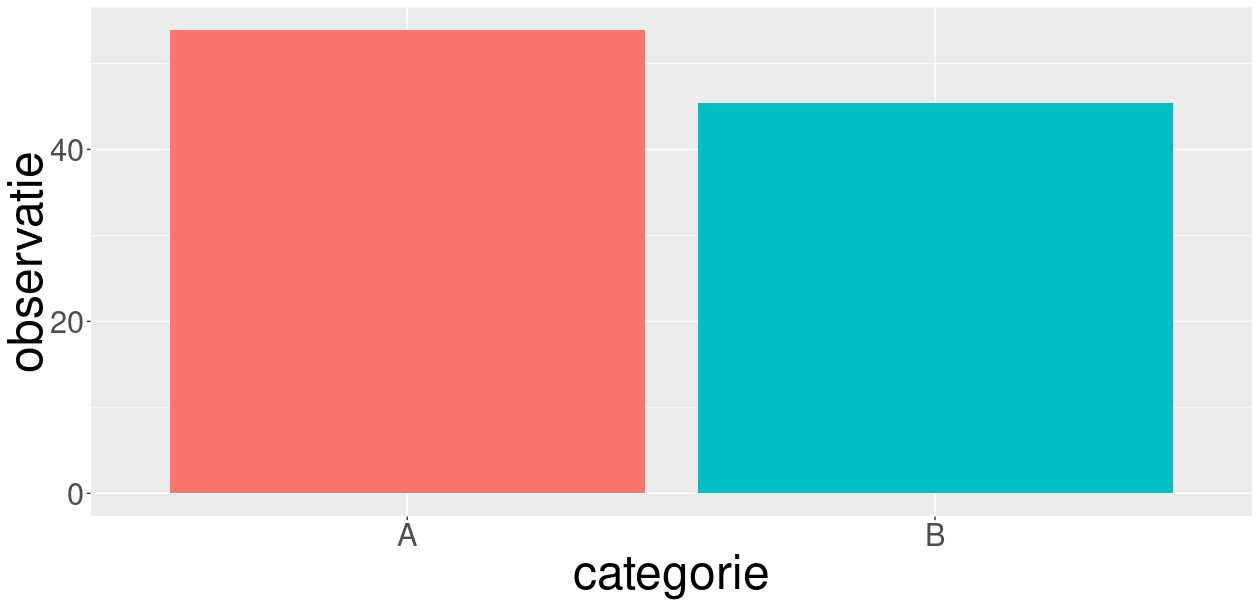
\includegraphics[width=\textwidth]{voorbeelden/barplot.png}
    \caption{Staafdiagram van gemiddelden. Dit is onvoldoende om een conclusie te trekken}
    \label{fig:barplot}
  \end{subfigure}
  \begin{subfigure}{.5\textwidth}
    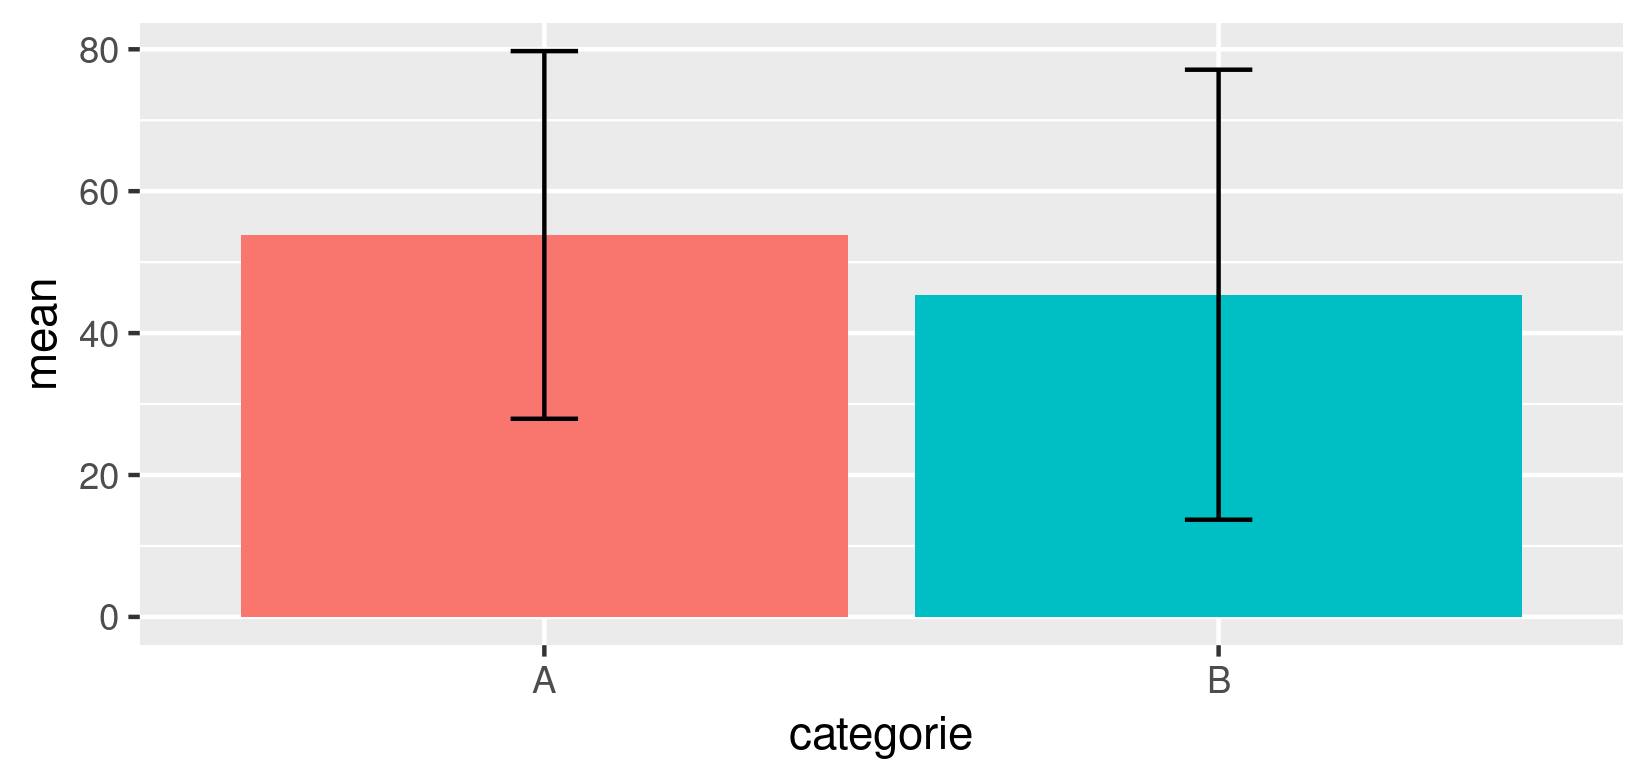
\includegraphics[width=\textwidth]{voorbeelden/barplot-errorbars.png}
    \caption{Staafdiagram met \textit{error bars} die de grootte van de steekproefstandaardafwijking voorstellen. Door de grote spreiding is het verschil tussen beide categorieën ineens veel minder uitgesproken.}
    \label{fig:barplot-errorbars}
  \end{subfigure}
  
  \begin{subfigure}{.5\textwidth}
    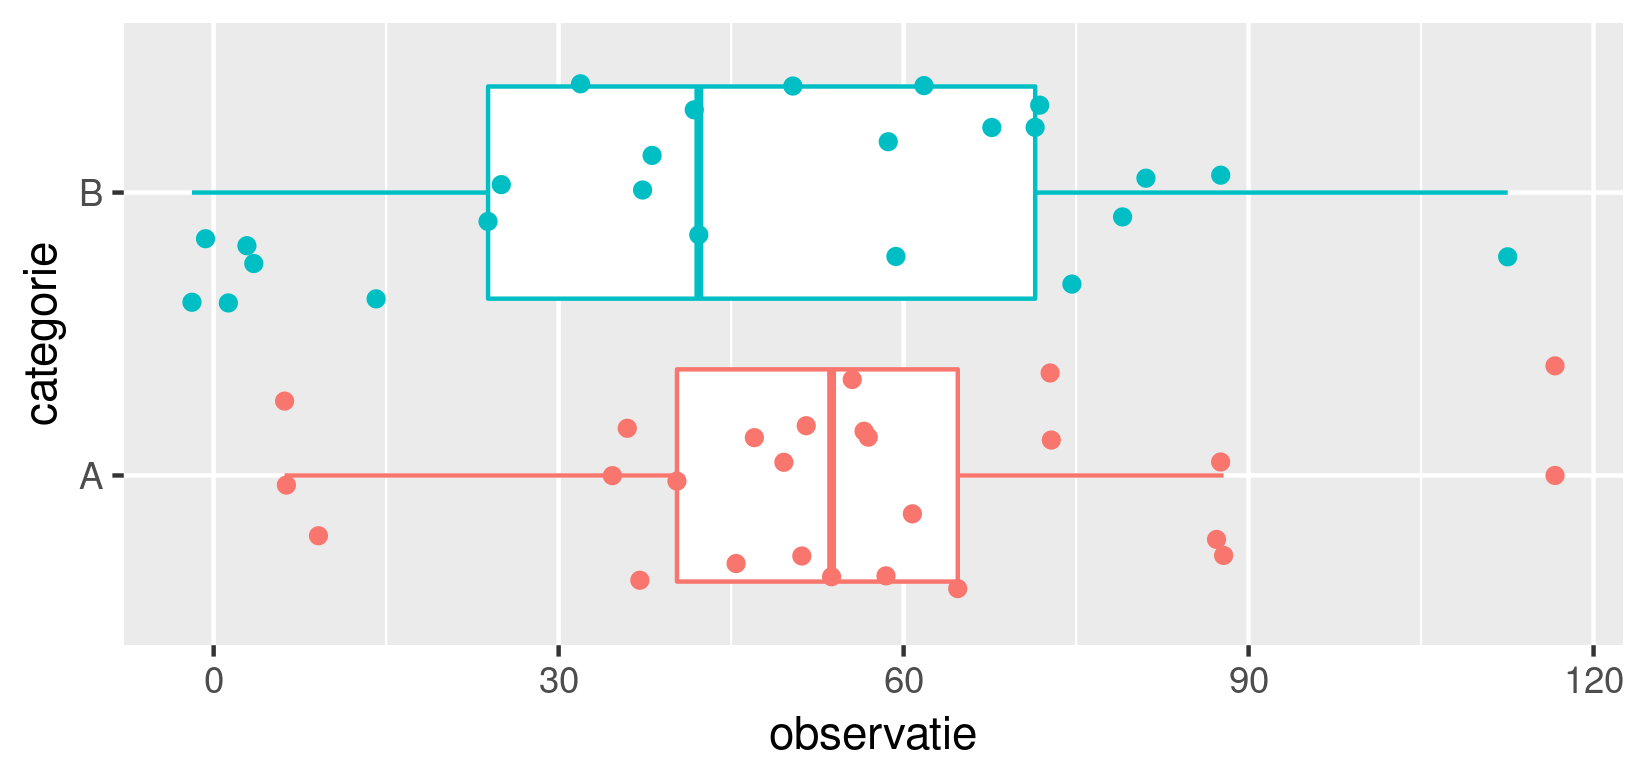
\includegraphics[width=\textwidth]{voorbeelden/boxplot-jitter.png}
    \caption{Boxplot met individuele observaties weergegeven als punten. Hiermee is de spreiding van de data nog duidelijker.}
    \label{fig:boxplot-jitter}
  \end{subfigure}
  \begin{subfigure}{.5\textwidth}
    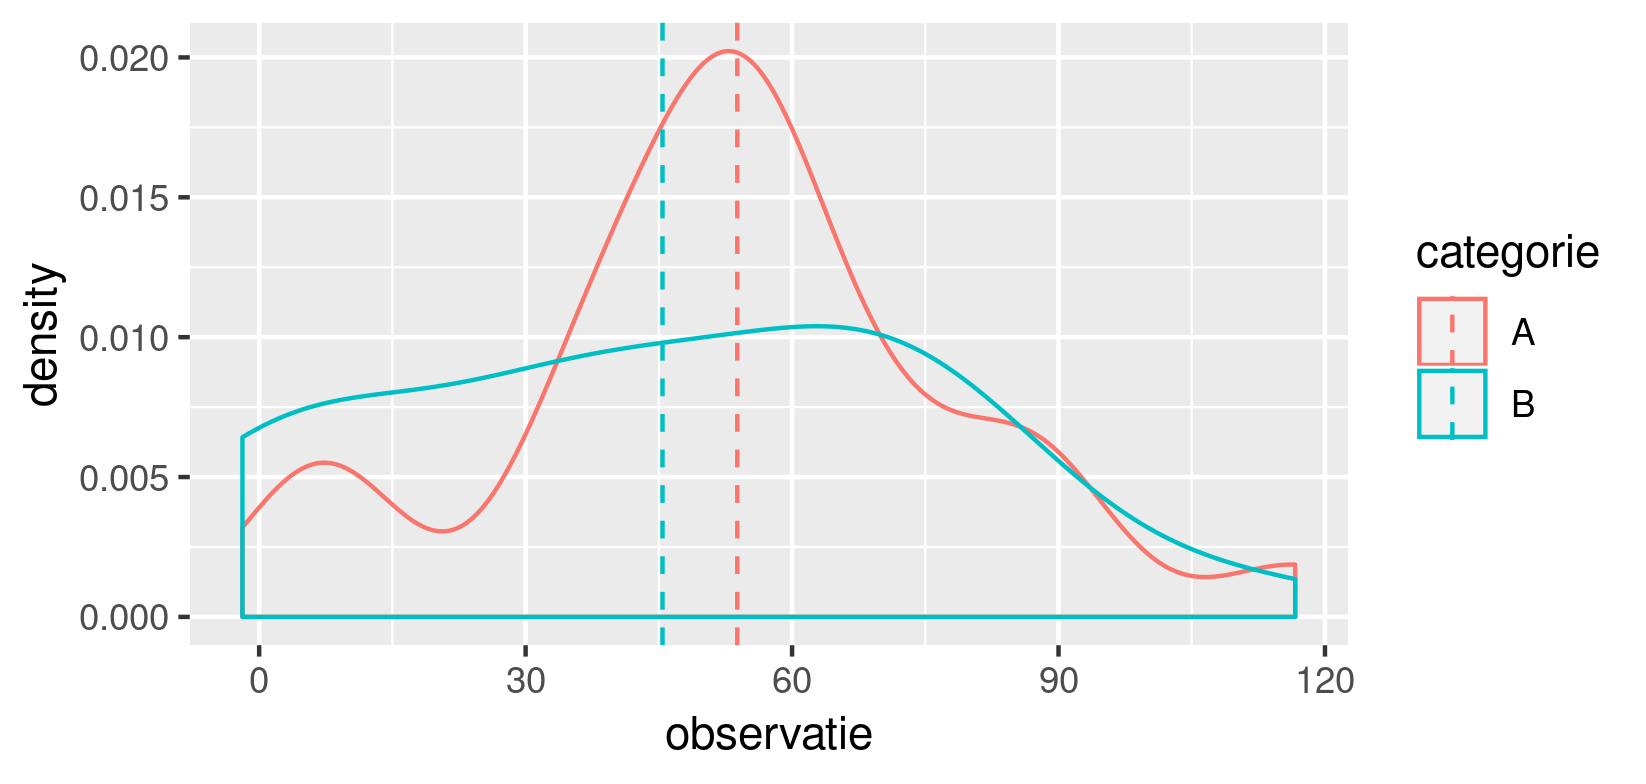
\includegraphics[width=\textwidth]{voorbeelden/density-plot.png}
    \caption{Kansdichtheid met steekproefgemiddelden aangeduid als een verticale stippellijn. Hier wordt duidelijk dat de resultaten van het experiment niet normaal verdeeld zijn. Dat maakt dat een staafdiagram met error bars eigenlijk niet geschikt is voor deze data.}
    \label{fig:density-plot}
  \end{subfigure}
  
  \caption[Visualiseren van cijfergegevens]{Verschillende manieren om dezelfde data te visualiseren.}
\end{figure}